\def\year{2020}\relax

\documentclass[letterpaper]{article} %DO NOT CHANGE THIS
\usepackage{aaai20}  %Required
\usepackage{times}  %Required
\usepackage{helvet}  %Required
\usepackage{courier}  %Required
\usepackage{url}  %Required
\usepackage{graphicx}  %Required
\frenchspacing  %Required
\setlength{\pdfpagewidth}{8.5in}  %Required
\setlength{\pdfpageheight}{11in}  %Required
\setcounter{secnumdepth}{0}  
\usepackage{subfigure}
\usepackage{multirow}

\begin{document}
% The file aaai.sty is the style file for AAAI Press 
% proceedings, working notes, and technical reports.
%
\title{Predicting Twitter Users' Political Affiliations Using Sentiment Analysis}
\author{Jabran Khan, Ridwan Sharif, Abdullah Sohail\\
\{ja6khan, r5sharif, a24sohai\}@uwaterloo.ca\\
University of Waterloo\\
Waterloo, ON, Canada\\
}
\maketitle


%%%%%%%%%. Introduction %%%%%%%%%

\section{Introduction} 

Social media platforms contain a wealth of information about the users on their platform, ranging from their behaviours to their interests. Users’ information can be explicitly stated, such as their taste in music or be implicitly stated, such as how risk averse they are. Many studies have shown that collecting and analyzing this data can help companies better understand their users. In turn, this information can be employed in a multitude of ways such as creating personalized adverts or even predicting the box office revenues of movies \cite{asurPredicting}. This paper will demonstrate how we can harness this data to infer a user's political leaning and anticipate voting patterns.

In this new age of information, classification systems that can determine political leanings are useful to efficiently allocate campaign finance, to determine where adverts and information should be directed and to aid in strengthening the democratic process. Analyzing the emotions and words people use is important to gauge the issues and policies that matter to the public.

Online social networks such as Twitter (our social media of choice) allows us to capture a snapshot of people’s sentiments about various issues at any given point in time. Building systems that can understand and analyze these sentiments about various issues can lead to larger administrative, political and societal changes.  In this paper, we discuss a methodology to mine the opinions and ultimately infer the political leanings of individuals. In doing so, we also explore the challenges involved, the scope and limitations of the system and the preliminary results and findings.

The main problem encountered when trying to determine the political leanings of a user is accurately analyzing the information available from their Twitter accounts. This information includes their tweets, retweets, hashtags and the users they follow. It is important to note that some tweets have no relevance to the user’s political beliefs, while others use negations or sarcasm which make it difficult to determine their overall sentiment.

To get around these limitations, we limit the scope of our analysis by selecting key topics that polarize users in order to create a strong differentiation within our tweet sentiments. Some examples of key topics include firearm regulations, abortion and climate change. We then compile a given user’s tweets and prune out tweets that are not related to the key topics. Afterwards, perform sentiment analysis on these tweets by utilizing a model that assigns sentiment values to words, such as assigning a positive sentiment to the word “love”. Following this, analyze the given user's sentiment across the key topics to determine their political leaning. For example, a positive sentiment with regards to gun control regulation indicates a left-leaning user. 

%%%%%Finally, this analysis is executed independently on a user’s followers and who they follow to validate our classification for the given user. The assumption made is that users are more likely to follow other users that share similar opinions \cite{himelboimBirds}. This means that if our results show someone is center-leaning but they follow and are followed by right-leaning users, then their political leanings should be adjusted to lean more towards the right. %%%5

%%%%%%%%%. Related Work %%%%%%%%%

\section{Related Work}

With the increasing popularity of social media and advancements made in computing fields, many studies have investigated text analysis techniques to gather information. Sentiment analysis is a popular process which mines a user’s opinions from a given text. Kharde and Sonawane discuss two approaches to sentiment analysis: lexicon-based and machine learning approaches. Lexicon-based analysis maintain a dictionary of opinion words which are used to determine a person’s opinion of a topic. In the case of machine learning, an algorithm is given a training set of data and generates a classifier that can determine (as best as it can) the opinion of the person. Kharde and Sonawane determined that lexicon-based approaches struggled to accurately predict a person’s opinion in comparison to machine learning algorithms, often performing over 10\% worse \cite{khardeSentiment}.

A lot of studies have focused on the relationship between politics and social media platforms. Political parties and government officials were quick to utilize sentiment analysis techniques to gauge the political opinions of users and to predict how it impacts the real-world political climate. Nausheen and Begum used a lexicon-based sentiment analyzer to predict election results based on the sentiment analysis of Twitter users. After assigning a sentiment to words, they trained a supervised classifier on each candidate in conjunction with 10,000 labelled tweets to determine the overall sentiment of each political candidate \cite{nausheenSentiment}.

Machine learning algorithms are a popular choice among researchers when performing sentiment analysis of user’s political preferences. Both unsupervised and supervised learning algorithms have been used. In one instance, an unsupervised learning method was used to determine the political stance of Twitter users by assuming that users are more likely to share the opinion of others that agree with them. Unsupervised learning was used to cluster users together based on their opinion of eight polarizing topics. Then, the pool of users was increased by training a supervised model on the remaining users to determine which cluster they belong to. With this stance data, they could determine the political stance of influential users and media outlets, achieving an 82.6\% accuracy on determining the stance of media outlets by comparing it to Media Bias websites \cite{stefanovPredicting}.

Supervised learning algorithms have been widely used and researched by many when determining political opinions. It is arguably the most straight-forward method since labels are given as part of the training set; the accuracy of such a model is easier to measure compared to that of an unsupervised learning algorithm which is not given labels \cite{khardeSentiment}. However, David et al. mention that creating labels is time consuming and may not be entirely accurate to how people view politics in real life. They suggest that rather than manually labeling texts, use a political party’s existing social media page to train the model instead; the party’s social media page can be classified as left or right. Using k-fold cross validation, a classifier can be made that can accurately determine a user’s political preference \cite{davidUtilizing}.

A glaring issue with using these sentiment analysis techniques is determining a person’s political preference using only words and their meanings. Languages are more complex. Users exaggerate emotions, use sarcasm, make spelling mistakes, use acronyms and more. Chung and Mustafaraj show that simple methods that analyze sentiments (from tweets) and predict election results are not much better than random classifiers. They hypothesize that the way to improve the models and the prediction results is to enrich the input data to include more than the polarity of words. They suggest that pre-processing techniques such as non-lexical features, POS tagging and word sense disambiguation might be necessary. Another big avenue that would improve the results is understanding context by looking at the user’s follower graph, past tweets, hashtags and more \cite{chungCan}. On a similar note, Maynard and Funk talk about the importance of a forward-looking approach when analysing user needs and interests. They do this by trying to understand people’s needs and interests in a more organic and general way such as drawing conclusions from their opinions about other products when predicting it about a similar one. According to them it is not enough to look at specific comments in isolation as associative information can dramatically change results \cite{maynardAutomatic}.

%%%%%%%%%. Methodology %%%%%%%%%

\section{Methodology}

Our application consists of several processing modules that combine to form a supervised learning pipeline that is able to determine a user’s political leaning. The different processing modules can be classified as follows:

\begin{enumerate}
	\item Topic selection
	\item Selecting and pruning tweets
	\item Building datasets
	\item Building the classification model
	\item Predicting political leaning
\end{enumerate}
Each of the following sections correspond to the steps mentioned above.

\subsection{Topic Selection}

As a part of gathering data to build our model, we select key topics that polarize left-leaning and right-leaning individuals. By doing so, we can minimize the number of tweets that are objective or neutral in nature, since it would be difficult to determine the sentiment for such tweets. Our main method to select appropriate political topics is to utilize census data gathered by the Pew Research Center in which they surveyed U.S. adults on key topics to determine which topics had the biggest political divide (\citeyear{pewresearch}). By utilizing census data, we take a data-driven approach to determining polarizing topics rather than guessing on our own, which reduces uncertainty in our model.

\subsection{Selecting and Pruning Tweets}

After the relevant topics are chosen, relevant users are selected whose tweets will be used as part of our training set. A user is a Twitter profile with over 100 tweets; we want the user to be sufficiently active on the platform to accurately determine their overall political affiliation. The more the user tweets, the higher the likelihood that they have expressed an opinion about a selected topic. Furthermore, only United States political figures and organizations are selected. Since we are focusing on U.S. politics, there is a much higher likelihood that the user will tweet about the policies that directly impact them and the U.S. Tweets unrelated to U.S. politics add noise to the training data and need to be disregarded.

For each selected user, only their tweets relating to the chosen topics are picked for the training set. This is done by searching for terms related to the topics. A simple program is built to increment through each tweet and selects the ones that contains one or multiple terms. Tweets with hashtags related to the topics are also selected. Hashtags are viable options because they are tracked, curated and displayed by Twitter. Hashtags are used by users to show support for their beliefs and the ideas that they associate with. There is little incentive for users to use hashtags for topics they do not support. Doing this ensures that irrelevant, noisy data is not present in the dataset.

While there are well known challenges of sentiment analysis that could affect our results, we have decided against pruning the tweets any further. The first challenge is deciding whether tweets that state facts should be removed from the training set since the sentiment of the tweet is more likely to be neutral. These tweets will not be removed from the training set because sentiment can still be derived from them. For example, the nomination of Amy Coney Barret can be stated either positively or negatively depending on the user’s political beliefs. Another challenge is that tweets contain complex language such as sarcasm and negations which can throw off the sentiment analysis. We will not be removing such tweets from our dataset. Our assumption is like that of \citeauthor{davidUtilizing} and their research. If enough tweets are collected, then a few sarcastic tweets will not heavily impact the resulting political affiliations of the users (\citeyear{davidUtilizing}). 

\subsection{Building Datasets}

\begin{figure}[t!]
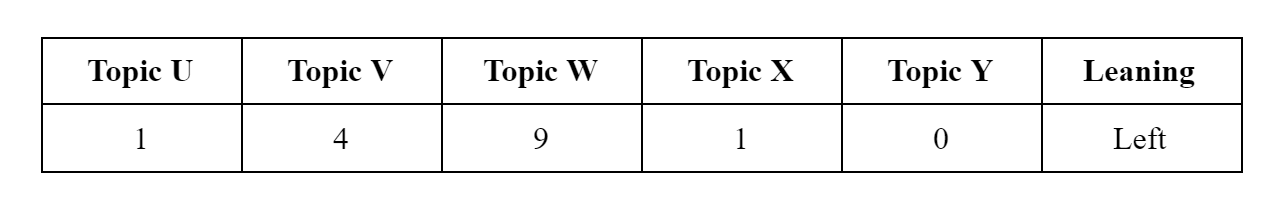
\includegraphics[width=8.5cm]{figures/table_row.png}
\caption{Individual User's Political Profile}
\label{fig:row_example}
\end{figure}

In order to build a supervised learning model, we need to gather data that we can train on. Similarly, we will need some data to test our classifier (described in the section below) and build confidence in our system. In order to do so, we will collect data and use k-fold cross-validation to make sure our system behaves optimally.

The dataset we are interested in is tabular in nature, where each row represents a user’s beliefs/sentiments about various topics and their political affiliation. After we’ve selected a set of topics (as described above), we measure the users sentiment (which is a real number value from 0 to 10 where 0 is negative and 10 is positive) on each of the topics and create a row in the dataset corresponds to the user’s political views. Each of the topics' sentiments serve as a real valued feature for the data and the result is a binary target (left or right leaning). These are the columns of the dataset. An example row in the dataset is shown figure \ref{fig:row_example} and is henceforth called political profile.

To build a political profile, we must be able to calculate real valued scores for users that represent their views on the given topics. For each topic, we prune all of their relevant tweets (as outlined above) and perform sentiment analysis on them. Then, we simply average their results and store them as shown above. The details of how we perform sentiment analysis are shared below:

To determine the sentiment of the tweets, we are using the Natural Language Understand API available through IBM’s Cloud platform. IBM has trained their Watson Natural Language Understanding using millions of text samples from various sources (such as the internet) over the past decade. They have developed one of the most accurate natural language processing models that is publicly available. Given a tweet and the corresponding topic, the API returns the sentiment of the text on a range from 0 to 10. Tweets with sentiment values less than 5 are labelled as negative while those with sentiment greater than 5 are labeled as positive. 

As for where we are collecting our dataset from, we were unable to find existing datasets that are readily usable. So instead we are collecting some data and creating our own. We are doing so by picking 1000 Twitter users (each user corresponding to a single row in the dataset) whose political affiliation is already well known. These 1000 users include the 100 pre-election senators, 434 house representatives, political pundits, talk show hosts, newspaper columnists and active political participants. Since our training/testing dataset of profiles is relatively small - we must carefully think about what kind of classifier we should use.

\subsection{Building The Classification Model}

Given the low cardinality of the datasets the system is training on, and given that the political leaning of an individual is based on the person’s sentiment about a slew of topics, our problem lends itself well to using a decision tree classifier. The different topics are real valued features and the political leaning is a binary target. An alternative model that could be used is a neural network. However, the reason we opted to go with a decision tree classifier is because the size of the dataset is relatively small and it can generalize the solution well. It also has increased flexibility and the ability to tune some of the decisions as we have visibility into what those decisions are. Finally, the decisions in the tree are very interpretable and can be visualized easily.

Each feature is a real-valued feature that represents the user sentiment about a given topic. In order to prevent overfitting and generate generalized and stable trees, we use the scikit-learn Decision Tree API. The API automatically determines the appropriate split-points for the features, plots the tree and generalizes well (using ensembling techniques for example). As mentioned earlier we will use k-fold cross-validation when training and validating the classifier before we use it to predict political leaning for arbitrary users.

\subsection{Predicting Political Leaning}

Once trained, our system accepts an arbitrary user’s Twitter handle. It then prunes the tweets relevant to the topics we have found to be most telling (with regards to their political leaning). It then performs sentiment analysis on the tweets of the user to generate a political profile for the user (as described above). Once this step is complete, we feed the profile to the classifier which then follows a sequence of decisions before arriving at a prediction about the user’s political leaning.

%%%%%%%%%. Results %%%%%%%%%

\section{Results}

As indicated by the final step of our algorithm, the goal of our research is to be able to take a user’s political profile and classify their political leaning. In order to ensure that our classifier is accurate, i.e. it does not overfit the training set we gathered from the 1000 Twitter users and is able to generalize to untrained data, we utilize tenfold cross-validation. We chose tenfold cross-validation instead of fivefold or some other number because this value was suggested as a general value that can be used to lower bias and variance \cite{khunApplied}. First, we start by shuffling the training set to make sure the data is evenly distributed, at which point we divide it into ten equal-sized segments. Next, we decide what parameter will be tuned. The machine-learning library we use is scikit-learn and it allows us to tune both the maximum depth (max\_depth) of the tree as well as the minimum number of nodes required to make a split (min\_samples\_split). Both of these parameters can prevent the tree from overfitting the training data, but we choose to tune min\_samples\_split due to a study by Mantovani et al. which suggests that a min\_samples\_split value between 1 to 40 works well for the algorithm scikit-learn uses to build the decision tree \cite{mantovaniAnEmperical}. For each of these 40 parameter values, we iterate over each segment in our shuffled training set, letting this segment act as the validation set V. The classifier is trained with the rest of the nine segments and then we run it on V, making note of what the prediction accuracy was. Since we do this for each segment, we are left with ten accuracy results in total, at which point we take their average to determine the overall accuracy for the given min\_samples\_split value. This means at the end we should be left with 40 average-accuracy values, and we choose the min\_samples\_split value that resulted in the highest accuracy. Finally, we pass the entire unsegmented training set to our classifier with our chosen min\_samples\_split value, giving us the classifier we use to determine a Twitter user’s political leaning.

The accuracy of the model developed is determined using classification accuracy. Classification accuracy is a simple metric which returns the ratio of the number of predictions made correctly to the total number of predictions made. It is a good metric to use for our model because our model solves a classification problem between two values, left or right. Precision, recall, and F1 Score are metrics we considered, but they are not necessary because the training set has an equal number of samples belonging to both classes. There is no risk of our model labeling in favor of one class since our traning is not skewed to either class.


%%%%%%%%% Bibliography %%%%%%%%%
\newpage
\bibliographystyle{aaai}
\bibliography{report}

\end{document}
